\documentclass{article}
\usepackage{import}
\subimport{../}{preamble}
\begin{document}

\section{Optical Design}

\begin{figure}[p]
\centering
\fontsize{9.5pt}{1em}\selectfont
\def\svgwidth{0.93\textwidth}
\subimport{./figures/}{layout.pdf_tex}
\caption[Diagram of the full optical layout]{\textbf{Diagram of the full optical layout and specification of the microscope.} All optics are accounted for except for silver periscope mirrors, which transfer the beam between platforms of differing height.}
\label{fig:layout}
\end{figure}

The optical design employs the concept of reimaging spatial filters into the correct planes for efficient spectroscopy leading to a compact design. Employing reimaging means that beams are not required to propagate exactly along the optical axis, minimising the number of long, empty beam lines, typically used for alignment. By reimaging the front and back focal planes of the objective, spatial and Fourier $k$-space filters are placed in the corresponding planes, ensuring optimum filtering performance and minimal aberration. A detailed schematic of the microscope platform and the surrounding optical bench layout, containing the specifications of all optics used, is found in \figurename~\ref{fig:layout}.

% Reimaging for compactness
Both image and Fourier planes are set through careful placement of each set of lenses. The required minimum degrees of freedom for beam alignment are accounted for by mirrors placed in the focal and Fourier planes. Those in the Fourier planes change the position of the beam without affecting the beam shape, whereas those placed in the focal planes only change the beam shape since the $k$-space distribution is changed by the angular deviation. The position and shape of the beam are therefore independently adjustable, greatly simplifying beam alignment. This advantageous technique results in high beam quality, and as a direct result of the lack of long, iris-containing beam lines, results in a compact microscope.

% The objective and illumination collar
A long working distance objective is required for imaging and spectroscopy. A \gls{bf} long working distance IR objective (Olympus LMPlan 100$\times$IR, 0.8\,NA) is used to access wavelengths above \SI{700}{nm}, for which the more convenient \gls{df} VIS objectives (Olympus LMPlan 100$\times$BD) exhibit a sharp cutoff. A dark-field illumination/collection configuration is necessary for spectrally studying scattered light from a nanostructure. Dark-field refers to the use of high-angle ($\mathit{NA}=n\sin\theta\geq0.7$) illumination, the reflections of which are filtered to collect only low-angle scattering from the focal plane. A large \gls{na} is required to properly study nanostructures in dark-field as it means light is collected across a large acceptance angle with a small focal length and large magnification. Since dark-field illumination is not supported on \gls{bf} IR objectives light needs to be brought in externally in a side-illumination geometry. A 3d-printed objective collar is used to hold a \SI{1}{mm} diameter optical fibre $\sim$1--\SI{2}{mm} from the sample, outside of the objective collection angle, to which a cold white LED is fibre coupled. The fibre is fed through a breadboard hole in the top plate and sealed so as to preserve the environmental chamber integrity. The fibre outputs a broad cone of light which illuminates samples over a large area.

% Fianium source
Use of a ultra-high brightness supercontinuum laser source (Fianium SC-400, \SI{4}{W}, 480--\SI{1750}{nm}) enables single nanostructure spectroscopy with exposure times on \orderof{\SI{10}{ms}}. The beam is expanded to fill the back aperture of the objective and apertured into a ring to mimic dark-field illumination using a dark-field disc stop. The inner diameter of the ring is set at \SI{2}{mm} and the outer diameter is set by the back aperture of the objective, in this case \SI{3}{mm}.
% Power control
Reflective neutral density filters totalling ND1.6 (2.5\% transmission) are placed in the beam line to reduce the incident power on the sample. The majority of the initial incident power is lost on the dark-field stop. Further attenuation results from the 10:90 (R:T) beamsplitter used to relay the laser into the microscope. At this point the power is reduced to \SI{1}{mW}, as measured on a bolometer (Coherent) behind the objective, to prevent laser damage to samples. Whilst the power is seemingly low and comparable with high-brightness incoherent light sources, the focussing ability of the single mode laser results in an intense, diffraction-limited, white light focus not possible with incoherent sources. Assuming a spot size on \orderof{\SI{1}{\micro\metre}} the focal intensity is on \orderof{\SI{e8}{mW\per cm\squared}}.

% Reimaging technique
The incident light is apertured and reimaged directly onto the back focal (Fourier) plane of the objective, as opposed to aperturing close to the objective back aperture, to prevent diffractive artefacts in the conjugate plane of the collected light. The ring aperture means that the focus is illuminated only at high-NA as with conventional dark-field spectroscopy. Scattered light is then filtered by the dark-field iris in the return beam path to collect only low-NA scattering, removing any signal contribution from reflected illumination.
Reimaging allows both the dark-field iris and stop to be located away from the objective for convenient access and easy adjustment. Alternative designs using optics mounted at the objective back aperture do not benefit from having the stop and iris in conjugate planes and may require motorised irises if not accessible by hand. For this experiment a simple graduated dark-field iris is sufficient for external use to filter the collected light signal.

% Collection efficiency
Since incident power is not an issue, and in many cases requires significant attenuation, the microscope is optimised for efficient collection. The 10:90 beamsplitter used for laser input means only 10\% of collected light is lost when returning back through the main microscope arm. Furthermore, all optics in the system are optimised for light between 500--\SI{1100}{nm}.\footnote{Achieved via exclusive use of Ag mirrors, Edmund Optics VIS-NIR AR coating on lenses, COMAR NIR and ThorLabs visible or visible-NIR coatings on beamsplitters} The angle-dependent Fresnel coefficients of the glass used in all optics components mean that $p$-polarised light is favoured during transmission.%
\footnote{All beamsplitters have some degree of polarisation sensitivity due to Fresnel coefficients of the glass used. Reflectance can be a factor of 2 different between orthogonal linear polarisations. For comparison of glass reflectances and Fresnel coefficients}
A \SI{90}{\degree} turning periscope is placed after the first reimaging lens to reverse the initial linear polarisations of light so that the axial polarisation with respect to the tip axis has highest transmission through the beamsplitters in the collection path.

Subsequently, collected light is split into imaging and spectroscopy paths using a second (50:50) beamsplitter placed before the dark-field iris.
% CCD imaging
CCD imaging is both used to align and characterise the laser focus and to centre samples onto the targeted laser illumination spot. Sample imaging uses light collected from the scattered side-illumination white LED light to produce dark-field images whereas the laser light is not \gls{df}-filtered in this path. Images are magnified 133$\times$.
% Spectroscopy - dark-field iris
Light passing along the spectroscopy path is filtered to remove any contributions from reflected light to the scattering signal. A graduated iris is used to remove the \SI{2}{mm} outer-ring (high-NA components) of the returning beam. The iris is placed in the image plane of the dark-field stop (Fourier plane) for the most accurate filtering and {\color{red}optimal/optimum} performance.
The two beamsplitters present before the dark-field iris are wedged to prevent ghost images, which transmit through the closed iris and create spectral artefacts. However, the \SI{5}{mm} thickness of wedged beamsplitters means increased dispersion and the limited availability of broadband AR coatings results in reduced reflectance in the NIR. %This, however, only affects CCD imaging, which is limited to visible wavelengths only.
Additionally, the \gls{df}-filtering process only works to remove light reflected out at the same angle. Angled samples (such as the facets of tips) can reflect light into the low-NA collection, creating more spectral artefacts. It is for this reason that the flat tip facets are even visible in a dark-field configuration.

%\subsection{Confocal Filtering}

% Confocal filtering
\begin{figure}[bt]
\centering
\fontsize{10pt}{1em}\selectfont
\subimport{./figures/}{confocal_diagram.pdf_tex}
\caption[Diagram of optical sectioning in confocal microscopy]{\textbf{Diagram of optical sectioning in confocal microscopy.} (a) Out of focus light from nearby reimaged focal planes leads to blur and a decrease of resolution in images. (b) Images spatially filtered in the focal plane by a confocal pinhole localise light from only a select volume that is sufficiently focussed to pass through the pinhole aperture.}
\label{fig:confocal_diagram}
\end{figure}

Since the laser focusses to a diffraction-limited spot on the sample, spectra are collected from a small sampling volume. Further spectral localisation is achieved by confocally filtering the image plane after the iris using a \SI{30}{\micro\metre} pinhole to collect light from only the central focal spot. Only light in focus on the pinhole may pass through it. By rejecting out of focus light the image becomes an optical section with a tight depth of focus. The size of the pinhole sets both the lateral and axial width of the transmitted in-focus light. The combination of spatial masking and optical sectioning creates a localised sampling volume in the objective-sample plane. This effect is shown in \figurename~\ref{fig:confocal_diagram}. The location of the spatial mask image, demagnified 53$\times$, in the objective focus, setting the sampling volume, is controlled by a mirror before the confocal filtering array. A slip-in disassembled webcam is used to image the Fourier plane before and after confocal filtering to measure the collection geometry. % should this go into the supplementary information?

\begin{figure}[bt]
\centering
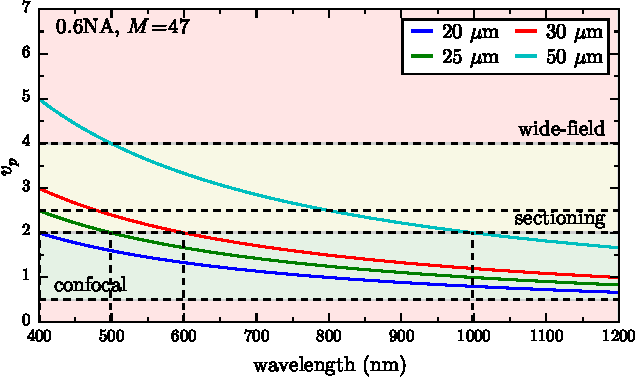
\includegraphics{figures/confocal_pinhole_choice}
\caption[Optimum confocal pinhole size across the visible-NIR spectrum]{\textbf{Optimum confocal pinhole size across the visible-NIR spectrum.}}
\label{fig:confocal_pinhole_choice}
\end{figure}

Confocal filtering not only improves the contrast but also improves upon the wide-field, diffraction-limited resolution by up to a factor of $\sqrt{2}$ at the cost of image brightness \cite{}. This is a result of the removal of higher diffraction orders by the pinhole thereby increasing the resolution. A decrease in the Rayleigh criterion \cite{} for diffraction-limited resolution, \gls{r_lat}, given by,
\begin{equation}
r_{\mathrm{lateral}}=\frac{1.22\lambda}{(\mathit{NA}_{\mathrm{obj}}+\mathit{NA}_{\mathrm{cond}})}=\frac{0.61\lambda}{\mathit{NA}},
\end{equation}
in expected in an epi-illumination geometry, to around,
\begin{equation} r_{\mathrm{lateral}}=\frac{0.37\lambda}{\mathit{NA}} \end{equation} \cite{}. The axial resolution, \gls{r_ax}, is also improved to,
\begin{equation} r_{\mathrm{axial}} = \sqrt{\left(\frac{n\lambda}{\mathit{NA}^2}\right)^2 + \left(\frac{\sqrt{2}nd_{p}}{\mathit{NA}}\right)^2}.\end{equation}
Decreasing the pinhole diameter not only decreases the thickness of the optical section but the minimum resolvable lateral distance. Since the depth of focus scales as $M^2$ the placement of the pinhole along the beam path is not critical. Choice of pinhole diameter, however, is important.

Realistically, however the detector is not a point detector but a finite aperture, so the collection \gls{psf} must be convoluted with the detector rect function, $D$, giving an image \gls{psf} $I=|h_1|^2(|h_2|^2\ast D)$. The FWHM of the image intensity retains the $\sqrt{2}$ improvement if the detector width $v_p\leq0.5$, but realistically this leads to a significant loss in brightness. Resolution is improved until $v_p\geq4$, at which point the wide-field behaviour is recovered. Practically $v_p\leq2$ to optimise lateral resolution and $v_p\leq4$ to optimise depth resolution. The optimum pinhole diameter is calculated using,
\begin{equation} \frac{M}{\mathit{NA}}\geq\frac{\pi d_p}{v_p\lambda}, \end{equation}
where \gls{pinhole} is the pinhole diameter. A sufficiently small pinhole diameter will have $v_p=2$, therefore for a 0.8\,NA, $M=53$ system $d_p/\lambda\leq45$, e.g. \SI{22}{\micro\metre} at \SI{500}{nm} and \SI{50}{\micro\metre} at \SI{1100}{nm}.

Since the incident laser illumination is not also confocally filtered, as required for idealistic point excitation, and exhibits a non-Airy diffraction pattern, a significant increase in resolution to the confocal limit is not expected. Confocal spectroscopy is moreso used for the lateral spatial localisation when studying extended nanostructures.

\begin{figure}[bt]
\centering
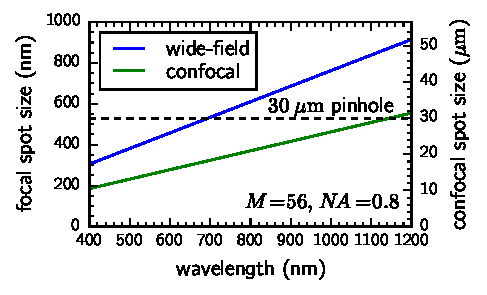
\includegraphics{figures/focus_spot_size}
\caption{\textbf{Magnified diffraction limited spot sizes for Gaussian beam focuses compared with the confocal pinhole diameter.} Larger wavelengths have larger focusses, therefore wavelengths with spot sizes greater than the pinhole diameter begin to get cut. Increased spatial localisation results in decreased spectral bandwidth.}
\label{fig:focus_spot_size}
\end{figure}

% Disadvantage is wavelength dependent focus size.
One limitation to the confocal technique is the choice of pinhole diameter. It is usual in confocal imaging to select a pinhole in terms of Airy units (A.u.). The width of the central maxima of the focus profile is defined as \SI{1}{A.u.}, to which the pinhole should be optimally between 0.5 and \SI{1}{A.u.}. The value of an Airy unit is wavelength dependent as it depends on the focus spot size, hence the pinhole will effect white light differently across the spectrum. It is assumed that the pinhole size is fixed at \SI{1}{A.u.} at a specific threshold wavelength. At the chosen threshold wavelength the pinhole behaves as expected. For wavelengths shorter than the threshold $d>\SI{1}{A.u.}$, therefore the whole diffraction pattern transmits, giving little benefit of confocal localisation. For wavelengths much larger than the threshold $d<\SI{0.5}{A.u.}$ and the throughput of light begins to decrease as the edges of the focus are cut. A drop in signal in the NIR is therefore expected.%
\footnote{This is also the case when focussing into a fibre.}
The pinhole parameters and focal spot sizes of an assumed Gaussian beam, taking account the magnification ($M=56$) from the sample plane to the pinhole plane, are shown in Figure~\ref{fig:focus_spot_size}. Use of a \SI{30}{\micro\metre} pinhole diameter was determined based on $k$-space images of beam structure {\color{red} (see below)}. The diameter sets \SI{1}{A.u.} at \SI{600}{nm} with cut-off beginning around \SI{800}{nm}.

% Spectroscopy in general
Once filtered only the spectral content of the beam is of interest rather than the image so strict adherence to conjugate planes is no longer necessary. The beam is split 50:50 into two signals, with one going to the benchtop spectrometers and the other to a fast spectroscopy path.%
\footnote{The fast spectroscopy technique is developed and implemented but otherwise not used in any experiments in the current project. For this reason it's operation is omitted from this work.}
% Spectroscopy arm
The benchtop spectroscopy signal is further split into linear $s$ and $p$ polarisation components using a broadband polarising beamsplitter cube (Melles-Griot 300--\SI{1100}{nm}). Broadband polarisers (Thorlabs 500--\SI{1500}{nm}) oriented along the $s$ and $p$ axes are placed at the cube output ports to increase the extinction. Each polarised signal component is then finally focussed into multi-mode fibres, using short focal length (\SI{11}{mm}) lenses to achieve a spot size smaller than the fibre core. \SI{100}{\micro\metre} fibre core is used instead of \SI{50}{\micro\metre} to reduce laser speckle in spectra since the \SI{30}{\micro\metre} confocal pinhole diameter already localises the signal.
% Spectrometers
The spectral signal from each of the fibres is recorded using TE-cooled, benchtop spectrometers (Ocean Optics QE65000 and QE Pro) with integration times on the on \orderof{\SI{10}{ms}}. The Si detectors in the spectrometers have a significant drop off in sensitivity beyond \SI{900}{nm}, imposing a limit to detectable signals of around \SI{1100}{nm}. The supercontinuum laser imposes as \SI{480}{nm} spectral cut-on, resulting in an effective measurement window of 500--\SI{1100}{nm}.

%\subsection{Measuring Spectra}
Measured spectra are background-subtracted and referenced to the spectral density of the supercontinuum illumination as transmitted through the microscope optics. Use of the intense supercontinuum source means low integration times of \SI{10}{ms} are usually sufficient for a high quality signal to noise. The high brightness of the supercontinuum laser with \SI{10}{ms} exposures also means that the relative intensity contribution from external light sources is negligible. Background subtraction is therefore mostly required to remove the dark counts inherent on the CCD.
The coherence of the supercontinuum laser means that conventional referencing using scatter from a white diffuser to map the illumination spectral density is not possible. Instead, reflections from a reflective substrate attached underneath the piezo-mounted sample mount are used as a reference. Different mirror substrates are used depending on the sample. For metallic samples the mirror substrate is matched to the metal so only structural spectral features are observed. Otherwise either a Ag mirror or glass slide are sufficient for referencing as they provide relatively flat reflectances across the visible-NIR spectrum.
The dark-field iris is kept fully open during reference acquisition to ensure the full spectral content of the incident beam is measured. A \SI{10}{ms} integration time is usually also sufficient to near saturate the spectrometer counts when acquiring reference spectra for maximum signal to noise. More signal than this (brighter reflections/longer integrations) requires further attenuation or iris closure, which is undesirable and can lead to spectral artefacts.
As optics are very rarely broadband between 400--\SI{1200}{nm}, all non-essential pathways are closed when acquiring spectra to prevent artefacts. Back reflections off lenses are found to superimpose a weak duplicate of the illumination spectrum onto spectra since the reflections are translated in $k$-space and are therefore not completely filtered by the dark-field iris.

\subsection{Characterisation of Microscope Performance}

% Power measurement
During most experiments the power incident on samples is kept below \SI{1}{mW} corresponding to a focal intensity of $\sim$\SI{e8}{\milli\watt\per\centi\metre\squared}. This is used to maintain sufficient signal quality whilst preventing damage or destructive changes to nanoscale Au samples (typically \SI{50}{nm} Au coatings).
% Beam profiling method
Beam profiling is used to characterise beam propagation in the microscope and determine its ability to collect dark-field spectra. Profiling is carried out using focal scans of both reflected light from a Ag mirror and scattered light from an \SI{80}{nm} AuNP, measured simultaneously on a CCD and a spectrometer. The CCD is used to laterally profile the beam through the focus while the spectrometer characterises the confocal profile and spectral distribution of the light. Both the illumination and collection pathways are profiled. The illumination pathway is profiled using the dark-field filtered supercontinuum beam while one of the collection fibres is removed from its spectrometer and is coupled with a \SI{532}{nm} single mode laser to profile the collection pathway.

\begin{figure}[bt]
\centering
%\fcapside[\FBwidth]
{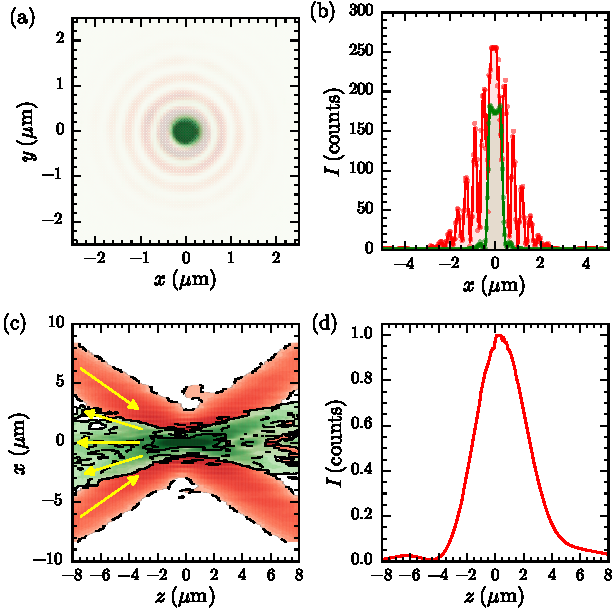
\includegraphics{figures/beam_profile}}
{\caption[Beam profiling of supercontinuum illumination and scattering collection beam lines.]{\textbf{Beam profiling of dark-field filtered supercontinuum illumination (red) and scattering collection (green) beam lines.} The spectroscopy pathway is characterised by coupling a \SI{532}{nm} laser into an single mode fibre and through the collection optics with the \gls{df}-iris closed to \SI{2}{mm}. Supercontinuum laser light is reflected back from a Ag mirror. The stated axial distance $z$ is twice the displacement of the mirror to account for reflections to the focal plane. Lateral distances are calculated using the CCD array size and pixel dimensions. (a) Lateral beam profile of the illumination and collection focusses as measured on the CCD. (b) Intensity cross sections through the lateral beam profiles of the illumination and collection. (c) Axial cross section through the focus of illumination and collection beams. (d) Normalised summation of spectrometer counts of confocally localised supercontinuum light passing through the collection optics.}
\label{fig:beam_profile}}
\end{figure}

% Discussion of beam profiling in terms of dark-field spectroscopy technique
\figurename~\ref{fig:beam_profile} shows both the lateral focal spot on the CCD and relevant cross sections along the optical and focal axes for both the illumination and collection optics, along with depth-profiling using broadband-integrated spectra. \figurename~\ref{fig:beam_profile}a shows the beam structure in the focus. The single mode fibre output has a Gaussian beam profile focus while the ring aperture of the supercontinuum beam achieves a tighter focus but with more power concentrated in its outer rings (\figurename~\ref{fig:beam_profile}b). The axial cross section of beams (\figurename~\ref{fig:beam_profile}c) shows the focussing of the high angle (0.71--0.8\,NA, 45--\SI{53}{\degree} incident angle) supercontinuum ring. The \gls{df}-iris restricts the collection angle of light from the focus to below $\sim$\SI{32}{\degree}, depending on closure extent, to reject the high angle supercontinuum components. After confocally filtering the depth of focus of the sampling volume is \SI{4}{\micro\metre} (\figurename~\ref{fig:beam_profile}d).
This could potentially be improved by confocally filtering the supercontinuum input to become similar to a true confocal microscopes. For most cases it is not necessary since samples are suspended nanostructures and depth profiling is not necessary.

% Axial chromatic aberration
\begin{figure}[bt]
\centering
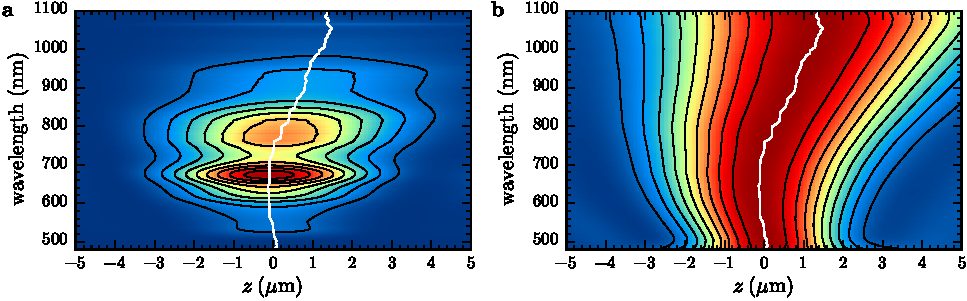
\includegraphics{figures/axial_chromatic_aberration} % maybe wants contour lines on to improve
\caption[Axial chromatic aberration at each wavelength through the objective focus]{\textbf{Axial chromatic aberration at each wavelength through the objective focus.} The image is formed from spectra of the $s$-polarised component of a reflection from a Ag mirror scanned through the focus. An intensity plot normalised for each wavelength is shown to determine depth of focus. The white indicates the position of maximum signal along the optical axis for each wavelength and shows the distinctive bowing curve of chromatic aberration.
%Each axial slice is normalised to the maximum wavelength.
}
\label{fig:axial_chromatic_aberration}
\vspace{-5pt}
\end{figure}

\figurename~\ref{fig:axial_chromatic_aberration} shows the individual wavelength components that make up the integrated spectral signal in \figurename~\ref{fig:beam_profile}d. As expected the depth of focus increases with wavelength. The depth varies from \SI{2.5}{\micro\metre} at $\lambda=\SI{500}{nm}$ to \SI{5.5}{\micro\metre} at $\lambda=\SI{1100}{nm}${\color{red}, typical values for confocal microscopes at these wavelengths \cite{}.} The chromatic structure of the beam is non-linear and shows that the colour maxima for $\lambda<\SI{550}{nm}$ and $\lambda>\SI{800}{nm}$ occur slightly offset from the pinhole position. Overall this does not detract much from the measured spectra since intensity differences in the chosen focal plane are normalised with the reference.

% AuNP hyperspectral scans show lateral localisation vs. pinhole diameter
\begin{figure}[bt]
\centering
%\fcapside[\FBwidth]
{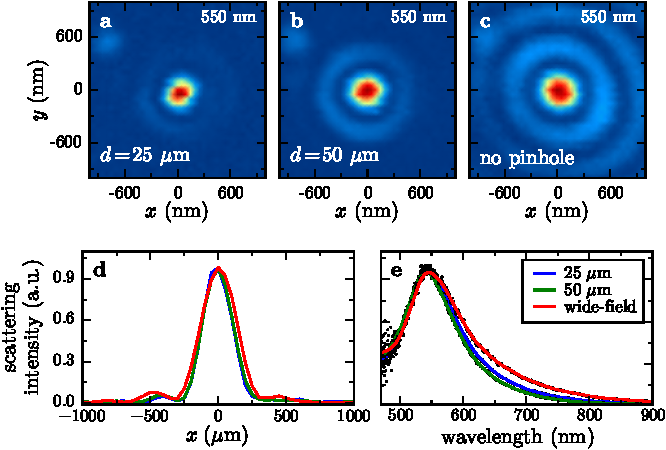
\includegraphics{figures/lateral_aunp_scans}}
{\caption[Hyperspectral scans of AuNPs used to characterise the lateral PSF with different confocal pinhole diameters.]{\textbf{Hyperspectral scans of AuNPs used to characterise the lateral PSF with different confocal pinhole diameters.} (a-c) Wavelength slices of AuNP scans on resonance using \SIlist{25;50}{\micro\metre} diameter pinholes and finally no pinhole, respectively. (d) The extracted PSF from line profiles across the images (a-c). (e) Spectra of AuNPs imaged. Localisation is observed as the concentric illumination rings are cut as the pinhole diameter is reduced.}
\label{fig:lateral_psf}}
\end{figure}

Lateral localisation is more important to consider than axial sectioning. The true lateral resolution is difficult to characterise due to the large broadband focal spot and its ringed structure. Scattered light from a sub-wavelength size nanoparticle provides a point source for measuring the \gls{psf} across a small, resonant bandwidth. The measured lateral scattering response of a confocally (raster-) scanned \SI{80}{nm} AuNP at it's resonant frequency, $\lambda_{LSP} = \SI{550}{nm}$, is shown in \figurename~\ref{fig:lateral_psf}. Images are acquired by raster-scanning over a grid containing a AuNP and measuring the spectrum at each pixel, from which a single wavelength slice is extracted. The confocal pinhole is replaced and the optics realigned between scans of the same AuNP.
Without a pinhole the image of the AuNP is a convolution of the supercontinuum light focal pattern (Figure~\ref{fig:beam_profile}a) and the AuNP scattering point source. It's spectrum is a convolution of its own plasmon resonance and the supercontinuum spectrum at each point in the pattern. The spectrum is normalised against the laterally-integrated spectrum of the supercontinuum laser reflected off a Au mirror to only show the plasmon resonance.
From the images (\figurename~\ref{fig:lateral_psf}a--c) it is clear that the addition of a pinhole restricts the spatial extent of the \gls{psf} by filtering the contribution of the outer illumination rings to the image. The pinhole diameter is reduced until only the central focus remains. Identifying this point becomes difficult as diffraction from the pinhole aperture blurs the focus in the focal planes after the pinhole. This occurs when using a \SI{30}{\micro\metre} pinhole, and is primarily why that diameter pinhole was chosen. Larger pinholes (only \SI{50}{\micro\metre} tested) let through a larger portion of the outer rings while there is no more gain in localisation from smaller pinholes (\SI{25}{\micro\metre} tested), instead losing only signal. The width of the central maximum in the PSF (\figurename~\ref{fig:lateral_psf}(d)) is also only marginally reduced between pinhole sizes so there is little gain in resolution.

% Lateral chromatic aberration as measured by monitoring the AuNP PSF vs. wavelength
\begin{figure}[bt]
\centering
%\fcapside[\FBwidth]
{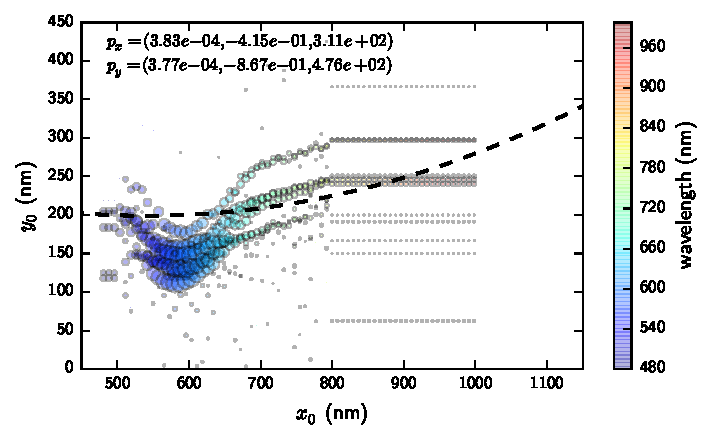
\includegraphics{figures/lateral_chromatic_aberration}}
{\caption[Measurements of lateral chromatic aberration across the plasmon resonance scattering bandwidth from hyperspectral images of AuNP.]{\textbf{Measurements of lateral chromatic aberration across the plasmon resonance scattering bandwidth from hyperspectral images of AuNP.} The central position of the scattering centroid is extracted from images at each wavelength. Changes in centroid position with wavelength signify chromatic aberration.}
\label{fig:lateral_chromatic_aberration}}
\end{figure}

Chromatic aberration in the scattering signal across the resonance bandwidth can also be determined from the hyperspectral image stacks. The central position of the scattering centroids are extracted from each of the wavelength slices in the hyperspectral image. Changes in the centroid position between wavelength images signifies chromatic aberration. The extent of chromatic aberration in the sample plane is shown in \figurename~\ref{fig:lateral_chromatic_aberration}.
% Why understanding the chromatic aberration is useful
Characterising this aberration, if systematic, means that the lateral position of wavelength images in the hyperspectral stack can be adjusted to correct for chromatic aberration. This has its advantages when recombining the individual wavelength images back into a colour image or colourmap.

% Summary
To summarise, beam profiling clearly shows that the supercontinuum dark-field technique works as expected and that spectra are collected from a small volume in the objective focus. This is significantly improved by implementing confocal microscopy to spatially localise spectra.

\FloatBarrier
\end{document}